\chapter[Bidding]{Calculating Bid Price}
\label{appendix-bid-price}

 In this section we model the return on an investment in urban properties. We model each agent as %'ll assume that all agents are
 speculating on potential \glspl{capital gain} as well as on the \gls{use value} they get from living in a property. %We assume that the use value is captured by the stream of rental values. %, whether a home is owner-occupied or held by an investor as a financial asset. 
 % For simplicity, we consider a one-period investment.  %To keep the analysis simple without loss of generality 

 The agent purchases a house for a price, $P_0$ %a down payment, $D$, 
 and receives the increased price $P_T = (1 + \dot P)P_0$, back after a period $T$. 
% The value of the investment is the net present value of buying and then selling after one period:
The value of the investment is the capital gain, $\mathcal{C}$ plus the rents, net of operating costs and taxes, $\mathcal{R}_N$.

% minus the mortgage, repaid with interest, plus rents, minus any operating costs and taxes,\footnote{We have applied this model to explore the effect of a vacancy tax in Beirut.  For that analysis we  added a use-value, $U$ in place of rent for expatriate owners to represent using the property - say one month a year - when they are not renting the property and a \textbf{vacancy tax}, $T$ at rate $t$ to affect the speculator's  decision.} %\cite{Al-Shihabi}

\begin{eqnarray}
V &=& \mathcal{C} + \mathcal{R}_N \nonumber \\
  &=& \mathcal{C} + \mathcal{R} - \mathcal{O} - \mathcal{T} \nonumber \\
  &=& \delta \left(P_T- \left(1+r\right)M\right) + \mathcal{R} - \mathcal{O} - \mathcal{T}.
\label{eqn-property-investment-value1}
\end{eqnarray}

% OLD equations from working out the above. Could change symbols
% \begin{eqnarray}
% V  	&=& capital\ gain - Interest\ due  	+ Rent  - operating\ cost -taxes\\
% 	&=& \delta P_T-D \qquad \qquad \quad - (1+\delta r)M \quad	 + R  	-C\\
% 	&=& \delta P _T \qquad-(P_0-M) \quad- (1+\delta r)M 	 + R  	-C\\
% 	&=& \delta (1+\dot P)  P_0 -(P_O -M)  -(1+\delta r)mP_0  + R  -C\\
% 	&=& \delta (1+\dot P)  P_0 -P_O + M \qquad -(1+\delta r)mP_0  + R -C\\
% 	&=&( \delta (1+\dot P)-1)  P_0  + mP_0 \quad -(1+ \delta r)mP_0  + (\rho-\kappa)P_0\\	
% 	&=& \left(  \delta (1+\dot P)-1    + m \quad - m(1+\delta r)  + (\rho-\kappa)\right)P_0\\'
% 	&=& \left(  \delta (1+\dot P)-1    + m \quad - m-\delta rm  + (\rho-\kappa)\right)P_0
% \end{eqnarray}

 Where $\mathcal{R}$, $\mathcal{O}$, $\mathcal{T}$, and $M$ are  net present values for rent, operating costs, tax payments, and the mortgage at the end of the period. The interest rate is $r$, and the discount factor $\delta$.

 For ease of calculation, this may also be written in terms of shares of the purchase price:
\begin{eqnarray}
V &=& \delta \left((1+\dot P) P_0 - (1+r)mP_0\right) + \rho P_0 - \theta P_0 - \tau P_0 \nonumber \\
  &=& \left(\delta \left(1+\dot P - (1+r)m   \right) + \rho     - \theta     - \tau\right) P_0.
\label{eqn-property-investment-value2}
\end{eqnarray}
 
 Where $\rho$, $\theta$, $\tau$, and $m$ are rent, operating costs, taxes, and mortgage shares. The net rent can also be written as a share, $\phi$ of the rent $\mathcal{R}_N = \phi \mathcal{R}$. % Where $\phi$ is a fraction that takes into account taxes and operating costs. 
 % of price for rents, operating costs, and taxes. %The discount factor is $delta$, $P_0$ is the property price at the time of sale. %$r$ is the interest rate paid, and $m$ is the share of the price taken out as a mortgage.
 %It has  seven  parameters, $\delta, \dot P, r, m, \rho, \kappa$ and $t$. The first four, $\delta, \dot P, r$ and $m$ are exogenous for the investor while $\rho$, $\kappa$ and $t$  are    %Operating revenue and costs $\rho, \kappa$ and $t$ are expressed as  present values. 

The rate of return on funds invested, $r_{return}$, is the value divided by the size of the down payment, $D$: 
%The rate of return is $v = \frac{V}{D}$. %For expat investors, we get a \textbf{decision rule}:
%\begin{enumerate}
%\item  if $v \geq a$ (with some private use?) with no rent,  don't bother renting. 
%\item If $v(no\ rent\ and\ tax) < a\geq v(with\ rent)$,  then  rent. 
%\item If $ v(with\ rent) \le a $,  then sell 
%\end{enumerate}\
\begin{eqnarray}
r_{return} 
  &=& \frac{V}{D}  \nonumber \\
  &=& \left(\delta \left(1+\dot P - (1+r)m\right) \ + \rho - \theta - \tau \right) \frac{P_0}{D}        \nonumber \\
  &=& \left(\delta \left(1+\dot P - (1+r)m\right) \ + \rho - \theta - \tau \right) \frac{P_0}{P_0-mP_0} \nonumber \\ 
  &=& \frac{\delta \left(1+\dot P - (1+r)m\right) \ + \rho - \theta - \tau }{1-m}.
\label{eqn-property-investment-return1}
\end{eqnarray}
Equation~\ref{eqn-property-investment-return1} provides a criterion for investors. Agents invest if if their expected return is greater than the target return, they are seeking:
\begin{equation}
r_{return} \geq r_{target}. 
\label{eqn-property-investment-return2}
\end{equation}

\section{Agent's maximum bid given the rate of return}

% Agents must compute the maximum bid price they are willing to pay.
To find how much investors will bid, we need to find the maximum price that they are willing to pay. They need a bid price. This is the maximum price that satisfies the criterion $r_{return} \geq r_{target}$ from Equation \ref{eqn-property-investment-return2}, in Chapter \ref{chapter-financialization} on Financialization. Where the return is the value over the down payment:
% Equation \ref{eqn-property-investment-return1} expresses the expected return on investment in terms of the  market price, $P_0$: 

\begin{eqnarray*}
 r_{return} 
   &=& \frac{V}{D} \\
   &=& \frac{\delta \left(1+\dot P - (1+r)m\right) \ + \rho - \theta - \tau}{1-m}.
\end{eqnarray*}

%which we define as the ``bid price'',% $P^{max}_{bid}$. 
The bid price is used in the price determination process in our model. %We return to Equation~\ref{eq:Value} %
replacing $\mathcal{R}$ with $rP_0$. 

\begin{eqnarray*}
V &=& \mathcal{C} + \mathcal{R}_N \nonumber \\
  &=& \delta \left(P^T- (1+r)M\right) +\phi \mathcal{R}
\end{eqnarray*}
% We also have to assume that $P^{bid}=P_0$, which we can justify as an equilibrium condition - investors believe they are paying the market price. The result is 
% \[V= \delta(P^T- (1+r)M)   +\phi r P^{bid}\]

%

The  price at the end of the term $T$,  $P^T$, is a predicted value  for the investor \textit{ex-ante}, so we have to replace $P^T$ in Equation~\ref{eq:Value} with a predictor, $(1+\dot P)P^{bid}$. 
\[V= \delta \left((1+\dot P)P^{bid}- (1+r)M\right) +\phi \mathcal{R}\]

Then we replace $\dot P$ with and estimate, $L(P)$, representing an estimated function of the lagged values of $P$ and any  other relevant data. We imagine the potential investor drawing on common  knowledge or information from the real estate agents or analysts.  The result is 
\[V= \delta \left((1+L(P))P^{bid}- (1+r)mP^{bid}\right) +\phi \mathcal{R}\]
Combining terms:
\[V= \delta \left((1+L(P))- (1+r)m \right) P^{bid} +\phi \mathcal{R}\]

WHY BIG BRAKETS NOT SHOWING UP

The rate of return $v=V/D=V/(1-m)P^{bid}$ is then

\[v= \frac{\delta \left((1+L(P) - (1+r)m\right)}{1-m} + \frac{\phi \mathcal{R}}{(1-m)P^{bid}}\]

% %++++++++++++++++

% \begin{align}  
%   v  & =  \frac{\delta ((1+\dot P)  - (1+r)m)\  + \psi r}{1-m}\label{eq:RULE}\\
%   & =  \frac{\delta ((1+\dot P)  - (1+r)m)\  + \psi r}{1-m}\label{eq:RULE}
% \end{align}

% \begin{eqnarray}
% v %&=& \delta(P^T- (1+r)M) \qquad \qquad \qquad 	 + \mathcal{R}_N \nonumber\\
% % &=&\delta\left( (1+\dot P)P^{bid} - (1+r)mP^{bid} \right)  + \mathcal{R}_N  \nonumber\\
%   &=&\delta\left( (1+L(p)) - (1+r)m \right) P^{bid} + \mathcal{R}_N  \nonumber
% \end{eqnarray}

The rule is, ``Bid if the RHS is larger than the target rate of return, $r^{target}$, and do not bid if it is smaller.''  The maximum bid is the bid that makes the two sides equal. 

\begin{align}
r^{target} &= \frac{\left[\dots \right]}{1-m}   +\frac{\phi \mathcal{R}}{(1-m)P^{bid}}. \\
%
(1-m)r^{target} &= \ \ \left[\dots\right] + \frac{\phi \mathcal{R}}{P^{bid}}\\%\delta(1+L(P))- (1+r)m%
%
(1-m)r^{target}-\left[\dots\right]  &=  \frac{\phi \mathcal{R}}{P^{bid}}\\
%
P^{bid} &=    \frac{\phi \mathcal{R}}{(1-m)r^{target}-\left[ \dots\right]}\\
%
P^{bid} &=    \frac{\phi \mathcal{R}}{(1-m)r^{target}-\left[ \delta(1+L(P)- (1+r)m\right]}
\end{align}

The denominator is an adjusted rate of return for capitalizing net rents, analogous to the value of $r$ in Equation~\ref{eq:Capitalization}. 


% \begin{eqnarray}%. OLD VERSION: WRONG
% %r^{target}&=& \delta\left( (1+L(p)) - (1+r)m \right) P^{max}_{bid} + \mathcal{R}_N  \nonumber\\
%    P^{max}_{bid} &=&\frac{r^{target} - \mathcal{R}_N}{\delta\left((1+L(p)) - (1+r)m \right)} %\label{EqBidPrice2} 
% \end{eqnarray}



% \section{Finding bid price}
% We start with Equation~\ref{B2}. for convenience, replace $\rho -\kappa - \sigma $ with $\mathcal{R}_N$ (net Rent). 

% Replace $P^T$ with $(1+\dot P)P^{bid}$ assuming that the bidder is bidding the equilibrium market price for the period.

% Then replace   $\dot P$ with $L(p)$ representing some (estimated function ($\tilde{\dot P}$)) of the lagged values of $P$ that incorporates other data. 

% \begin{eqnarray}
% v&=& \delta(P^T- (1+r)M) \qquad \qquad \qquad 	 + \mathcal{R}_N \nonumber\\
%  &=&\delta\left( (1+\dot P)P^{bid} - (1+r)mP^{bid} \right)  + \mathcal{R}_N  \nonumber\\
%   &=&\delta\left( (1+L(p)) - (1+r)m \right) P^{bid} + \mathcal{R}_N  \nonumber
% \end{eqnarray}

% So I want to use this relationship to find the maximum bid price for the bank. The rule is, ``Bid if the RHS is larger than the target rate of return, $r^{target}$, and do not bid if it is smaller.''  The maximum bid  is the bid that makes the two sides equal. 

% {\color{red}
% \begin{eqnarray}
% r^{target}&=& \delta\left( (1+L(p)) - (1+r)m \right) P^{max}_{bid} + \mathcal{R}_N  \nonumber\\
%    P^{max}_{bid} &=&\frac{r^{target}-\mathcal{R}_N}{\delta\left( (1+L(p)) - (1+r)m \right)} \label{EqBidPrice} 
% \end{eqnarray}}
% %(What makes. this work is that I do not use an identity to get $\dot P$, which made the system of equations singular.)
% \newpage

\section{Other factors affecting price determination}
% \subsection{On bidding}

In practice, potential investors will make an  initial  bid that is lower than this value and subsequent bargaining will settle of a price between the initial bid and the seller's asking price.

In the market, the initial bid should be smaller than the bid price calculated, which is a maximum that can earn the target rate of return, The bank will definitely go this high. 

If there is a  max bid among competing buyers, the second highest max bid should be the sale price, but the bidder with the highest max bid wins the property. This makes sense because in a bidding war the final bid only has to be a very small amount higher than that of the last competitor left.
That is the highest price that a seller can get.

It might be simplest to treat every seller as a bidder. All bid above her own are considered. The seller chooses the second highest bid. This  seems realistic enough and is very simple to implement. It should producer a path that is indistinguishable form any more complex approach. 

Will persons retiring who would leave the city invest in an urban rental?

Bargaining between buyers and sellers differs. Buyers bid low and sellers ask high. {\color{red}We need to calculate a minimum selling price for the seller}.

% But what is $D$? Does the bank have unlimited funds? Isn't D just a fraction of P?  If so it cancels out
% r is the prime rate- that the bank pays? 


\section{Relating the bid price parameters to the code}

In the following sections we discuss the computation of agents' bid price, outline potential discounting approaches, and discussing how each component of the calculation is treated in the code. 

Agents calculate their bid price following the logic in Equation~\ref{eqn-bid1}: 
% \begin{align}
% P^{bid} \le   \frac{ \mathcal{R}_N}{(1-m)r^{target}-\left[ \delta(1+L(P)- (1+ r)m)\right]}. \nonumber
% \end{align}
% Or with individual subscripts
 
\begin{align*}
P_i^{bid} \le   \frac{ \mathcal{R}_N}{(1-m_i)r_i^{target}-\left( \delta_i(1+L(P)- (1+ r_i)m_i)\right)}. 
\end{align*}

This equation is introduced in section. 
Agents borrow a share of the purchase price, $P$. The amount borrowed is the mortgage, $M$. This is a share of the total purchase price $mP = M$
The \gls{mortgage term}, $T$, is the period it takes to pay down the mortgage.

In the following subsections, we discuss each of the terms and how they are implemented in the code. Net rent, $\mathcal{R}_N$, is discussed in subsection \ref{SS:NetRent}. The borrowing ratio, $m_i$, is discussed in section \ref{SS:BorrowingRatio}, the target interest rate, $r_i^{target}$, is discussed in \ref{SS:targetr} the discount factor, $\delta_i$ is discussed in section \ref{SS:discountfactor}. The price approximation mechanism, $L(P)$ is discussed in \ref{SS:PriceForecast}, and the interest rate the buyer has to pay for the mortgage, $r_i$, is discussed in \ref{SS:BankRate}. Sections are thus numbered: 

\begin{align*}
P_i^{bid} \ge   \frac{\ref{SS:NetRent}} {(1-\ref{SS:BorrowingRatio})\ref{SS:targetr}-
\left[ \ref{SS:discountfactor}(1+\ref{SS:PriceForecast}- (1+\ref{SS:BankRate})\ref{SS:YWealthConstraint})\right]}. 
\end{align*}

In developing the model we introduced a number of rates, such as $r_i$, the rate that individual $i$ pays for a single borrowing period. The payment calculation is made for a period of length $T$, which we refer to as a mortgage term.
%This means the actual interest paid is a compounded interest rates (VARIABLES LIST FOR THIS).

%In developing the theoretical model we introduced a number of rates, such as $r_i$, the rate that  individual $i$ pays for a single period of borrowing. We assume the calculations are for a  period of length  $T$, which we refer to as a mortgage term. This means that the rates in equations such XXXXX are actually compounded rates.
Taking a simplified example, if the rate is $x$/year, interest payments are $xM$, a share of the total mortgage amount borrowed, $M$, for each of $T$ years. 
If the interest payments are all made at the end of the mortgage term, the lender will require interest on the deferred interest, so agent $i$'s payment at the end of the period $T$ will be:

\begin{align*}
\text{Payment} &= (1+r_i)M                                            \\ 
    &= M + xM(1+x)^{T-1}+ xM(1+x)^{T-2}\dots + xM(1+x)^{0} \\
    &= M\left(1+ x\sum_{z=T-1}^0(1+x)^{z}\right).          \\ 
\end{align*}
Therefore, the interest payment is:
\begin{align*}
r_i.   &=x\sum_{z=T-1}^0(1+x)^{z}.
\end{align*}

For the sake of notational simplicity and clarity of exposition,  we omit the compounding formula throughout our discussion. This means that, while banks may quote a per period interest rates, the equations use a compounded rate. In the computational model we employ the appropriately compounded values. All %the rates are compounded in this way to provide a per-period rates, including all 
 the interest rates, the $r$'s, are compounded in this way, because they require annual or monthly payments at their stated rates.
 It does not affect the discount rates, the $\delta$'s, or the borrowing ratio $m_i$, because they are initially calculated for the term and don't require the same period payments.
 The discount factor $\delta_i$ is always a compounded version of $x$:
 \[\delta_i=\left(\frac{1}{1+x}\right)^T\].
%is a feature of the individual, so it is not affected in this way.
%The appropriate compunding expressions for other rates are displayed below.

The {mortgage term}, $T$, is the period it takes to pay down the mortgage. We work with a mortgage terms for two reasons. First, in the theoretical analysis, by transforming the multi-period transaction to a single period, we simplify the comprehensibility of the analysis. Second, it reflects the fact that in practice agents  likely consider the profitability of a purchase for a finite term longer than one period. The term period lets them consider the time cost of money in their analysis in a natural way. Parameters for their discounting rates and the term considered can be used to explore the effect of borrowing costs and their personal discounting rates on their decisions. Future interest rates are also not fully known. In the future, we can also vary the compound interest rates to explore the impact of uncertainty, given agents' individual guesses about the future, and their level of risk aversion.



\subsection{Net rent}\label{SS:NetRent}

We assume that the present value of $\mathcal{R}$ is known to an investor in advance. We can imagine the investors' accountant having information on the rent that the market will bear or on prior rents and including this information in the calculation of $P^{bid}$.

Uncertainty can be represented as bias or stochasticity.
Calculation notes: I have rent from the wages. I have kappa and sigma from our ex parameter values. . omega from the wages. 

$\mathcal{R}_N = \phi \mathcal{R}$

Where the \gls{rent share}, phi is a fraction
$\phi = (rent-taxes-costs) /rent$ 

There's a distinction between the warranted rent, the net rent, and the rent that's actually charged.

We assume that the  rent  actually charged to a tenant is the warranted economic rent, ($\mathcal{R}= \omega - \tau d_j$), but the relevant term to enter into the calculation of return on investment is the net rent $\mathcal{R}_N$ for a given property, because the returns are the returns an investor can get after paying taxes and operating costs.

In our computational model, we do the calculation in terms of a mortgage, so we want the total returns after expenses, in present value, compounded over the mortgage  period.
% We want the total returns after expenses, in present value, compounded over a 5 year period.

\begin{align}
\mathcal{R}_N &= \mathcal{R} - \Theta - \Sigma 
\end{align}

In terms of the warranted rent, 
\begin{align}
\mathcal{R}_N &= (1-\kappa_j - \sigma_j)(\omega - \tau d_j)
\end{align}

% $\mathcal{R}_N = (1-\kappa_j - \sigma_j) (\omega - \tau d_j)$

% {\color{red}
% Notice that  we need here is really the fraction of the warranted rent that the owner gets to keep after maintenance costs and taxes. It is possible that the owner is charging more or less than the economic  rent, but economic rent can be seen as an equilibrium value. Economic rent is $\mathcal{R}$.  This is (tautologically) related to the price as a fraction of the actual sale price: COULD MOVE TO THE CHAPTER NOW SINCE THE THE SECTION IS MOVED THER
% }
% \[\mathcal{R}= \frac{\mathcal{R}}{P_0}P_0 \]

If we want to know the  present value  of the \textbf{net rent}, $\mathcal{R}_N$  collect over the period  $T$, $\mathcal{R}_N^T$, we \textbf{add up} the discounted rents for each year. We may assume the rents are rising at and that the first is the current warranted rent, which gives us a computational formula. 
\[\mathcal{R}_N^T= (\omega-\tau*d)\sum_{t=0}^{t=T-1} \frac{(1+\dot{\mathcal{R}})^{t}} {(1+r_{r_\delta})^{t+1}} \]

% \[\mathcal{R}_Nj^T= (\omega-\tau*d_j)\sum_{\tau=0}^{\tau=T-1}\left[\frac{1+\dot{\mathcal{R}}}{1+r_{r_\delta}}\right]^\tau \]
\noindent where $\dot{\mathcal{R}}$ is an expected rate of change of rents - possibly zero for now, and $r_\delta$ is the individual's discount rate. 

TODO: problem - how to handle subscripts with net rent $\mathcal{R}_N$



\subsection{Borrowing ratio}\label{SS:BorrowingRatio}
$m_i$

The borrowing ratio, $m_i$, is just the fraction of the price that the bank will lend to a potential buyer. \textbf{It may depend on the individual.} 

Income(\ref{SS:YWealthConstraint}) and/or wealth (\ref {SS:MWealthConstraint}) may constrain individual participation in markets. 
Here we should use the same logic as we use about the interest rate charged. (\ref{SS:BorowingRate})

It is likely to be higher for institutional buyers  and for the wealthy because the bank thinks those with assets are more secure risks. they may have other assets that could be attached in the case of default.
(note interventions with reduces interest rates, or loan assessments drawing on techniques used by foundations could have value)


\subsection{Target interest rate}\label{SS:targetr}

 The target interest rate, $r^{target}$, is the prime rate plus a margin. % required by the bank.  Question: do non-bank actors have such a term?

\begin{verbatim}
self.get-target-interest-rate(buyer)
\end{verbatim}



\subsection{Discount factor}\label{SS:discountfactor}

The discount factor $\delta_i$ for THE END OF period $T$ captures the cost of waiting $T$ periods to sell the property. The usual way to treat it, which we use here, is to assume that $i$ has an interest rate $r_i$ and has been investing efficiently. This means that  the individual has a discount factor for future returns based on the year-over-year rate of return. 

\[\delta^T_i=\left[\frac{1}{1+r_i}\right]^T\]



\subsection{Price forecast approximation} \label{SS:PriceForecast}
$L(p)$

$p$ is all the price data plus any exogenous information (EG Policy knowledge?). $L(p)$ is an estimation function that produces a `common knowledge' value for the rate of price increase. Later you can add idiosyncratic extra knowledge or extra ignorance.



\subsection{Prime interest rate}\label{SS:BankRate}
$r$

The bank's interest rate, $r$, is just the bank rate (prime rate? set by the Bank of Canada. Exogenous. Just assign  a value like 4\%.



\subsection{Other}
\subsubsection{Tax ratio}\label{SS:taxratio} 
The tax ratio $\sigma$ is the share of rents that the municipality takes for services and infrastructure. This fraction of the value of the property is about 30\% based on mill rates in Ontario,  so $\sigma = 0.3$. % REFERENCE

*** CHECK Total taxes paid on  property $j$, over a given mortgage period $T$ is 

\[\Psi_j^T = \psi * \mathcal{R}\].  



\subsubsection{Cost tax ratio}\label{SS:costratio} 
The value of $\kappa$  varies for every property based on maintenance requirements, historic rents, tenant rights, and variations in assessed values. If it varies, it may be useful as a quality indicator.

%Values for $\kappa$ and $\sigma$ must be adjusted to take into account the length of the period or net rents have to be summed over the period.  NO LONGER NEEDED 

Nothing prevents $\sigma+\kappa >1$, which would leave an investor unable to cover building maintenance and taxes out of current rent. 



\subsubsection{Wealth constraint on m} \label{SS:MWealthConstraint}


I have suggested that the availability of  capital is known to differ for rich and poor. 
The bank, as a person has lots of assets, so $m_i$ is close to one, say 0.9. 

For the median wealth holder, $m_i$ should be around - let's say, 0.8 and  
We need a function that captures this relationship so we need to define individual wealth:
\[W_i= P_i -M_i  +S_i\]
where 

\begin{tabular}{ll}
$P_i$ & value of owned home\\
$M_i$ & Mortgage on owned home\\
$S_i$ & personal savings = $age*d*W$\\
\end{tabular}


We first tie the borrowing \textbf{ratio}, $m_i$,  for agent $i$, to individual wealth. Figure~\ref{Fig:Borrowingratio} illustrates a mortgage availability  model that is written 
 \[ m_i = 0.1(9-\left(\frac{W_i}{\bar W}\right)^{0.5}/2 )\]
Where $\bar{W}$ is mean wealth and $W_i$ is individual wealth. 

\begin{figure}[htb]
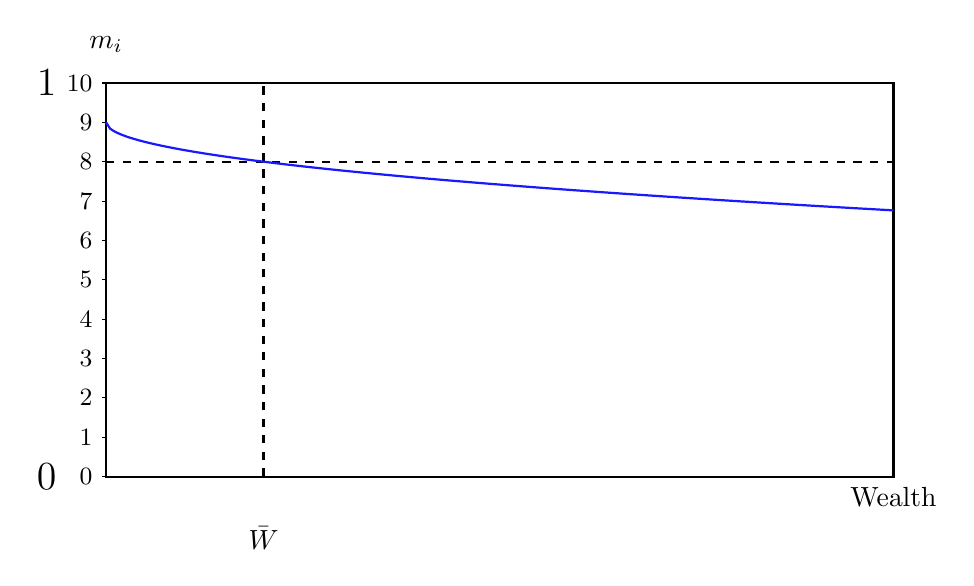
\begin{tikzpicture}[scale=.5]
%\def\bndmax{5}        %https://tex.stackexchange.com/questions/68462/filling-a-complex-region-with-tikz
%\def\bndmin{0.2}
\def\Y{10}  % height of y axis pecent
\def\W{20}  % length  of x axis
\def\Wbar{4}
\def\rbar{8}% this is the prime rate

% %Equation   \[ r_i = (A + .5 \frac{\bar{W}}{W_i})\omega\]
   % \def\Wmin{.63}  %This sets the lower limit fo the 
    \def\Wmin{(\B*\Wbar)/(\Y/\rbar-\A)} %function to keep in in bounds
	
 \tikzset{func/.style={thick,color=blue!90}}	

 \draw [thick](\W,\Y)-- (0,\Y)node[left=.5cm]{\Large$1$}node[above=.25cm]{$m_i$} -- (0,0)node[left=.5cm]{\Large$0$}--(\W,0)node[below]{Wealth}--cycle;  	% Axes box
 
 \draw [dashed, thick] (0,\rbar) -- (\W,\rbar);  	% Axes
\draw [thick,dashed] ( \Wbar,0)node[below=.5cm]{$\bar{W}$} -- (\Wbar,\Y);  	% Axes

\foreach \yi in {0,...,\Y} \draw (0,\yi)--(-.1,\yi)node[left]{\small$\yi$};
%\foreach \yi in {0,2,4,6,8,10} \draw (0,\yi)--(-.1,\yi));
%node[left]{\small$\yi$};
%\foreach \yi in {0,2,4,6,8,10}node at (-.1,yi) {{10*yi}} ;
\draw[func,domain=0:\W] plot [samples=200] (\x,(9-\x^.5/2);

 \end{tikzpicture}
\caption{Individual borrowing ratio $m_i$ as a function of wealth (in tenths)}
 \label{Fig:Borrowingratio}
\end{figure}


\subsubsection{Individualized borrowing rates}\label{SS:BorowingRate}
 
 
 $r_i$ depends on relative income and assets, as well as base interest rates. % compared to others. 
 The median after-tax income of Canadian families and unattached individuals was \$66,800 in 2020 according to Statistics Canada's %\href{https://www150.statcan.gc.ca/n1/daily-quotidien/220323/dq220323a-eng.htm}{Canadian Income Survey, 2020}.  \href{https://www150.statcan.gc.ca/t1/tbl1/en/tv.action?pid=1110005501}
 Data released in 2020 by Statistics Canada indicates that the top 1\% of Canadians made, on average, around \$512,000 in a single year \cite{stats-can-canadian-incomes}. % \href{https://www150.statcan.gc.ca/n1/daily-quotidien/201222/dq201222b-eng.htm}{Survey of Financial Security, 2019}.

 A study by Statistics Canada found that the typical Canadian household now has a median net worth of \$329,900, while the average net worth in Canada is \$738,200 \cite{stats-can-median-net-worth}.  %\href{https://www150.statcan.gc.ca/t1/tbl1/en/tv.action?pid=1110005501}{High income tax filers in Canada}

\subsubsection{Computing the income constraint on interest rates}\label{SS:YWealthConstraint}
$r_i$

In our model, we  tie the individual cost of capital,  $r_i$ for agent $i$, to a prime rate, $\bar r$ or the bank's target rate, $r^{target}$, prime plus 1\%, say. and to individual wealth. Figures~\ref{Fig:Borrowingrate1} and ref{Fig:Borrowingrate1} illustrate a couple of possible  cost-of-borrowing models roughly consistent  with the stylized facts about lenders. 

\begin{align}
 r_i =  &  \left(A + B \frac{\bar{W}}{W_i}\right) \bar r       \label{eq:incomeandr1}  \\
 r_i =  &  \left(\bar r - A + B *\frac{\bar W}{W_i - C}\right) \label{eq:incomeandr2}  \\
\end{align}
Where $\Bar{W}$ is mean wealth and $W_i$ is individual wealth. In Equation~\ref{eq:incomeandr2},  A determines y-shift, B, the scale, and C the  x-shift for the curve.


\begin{figure}
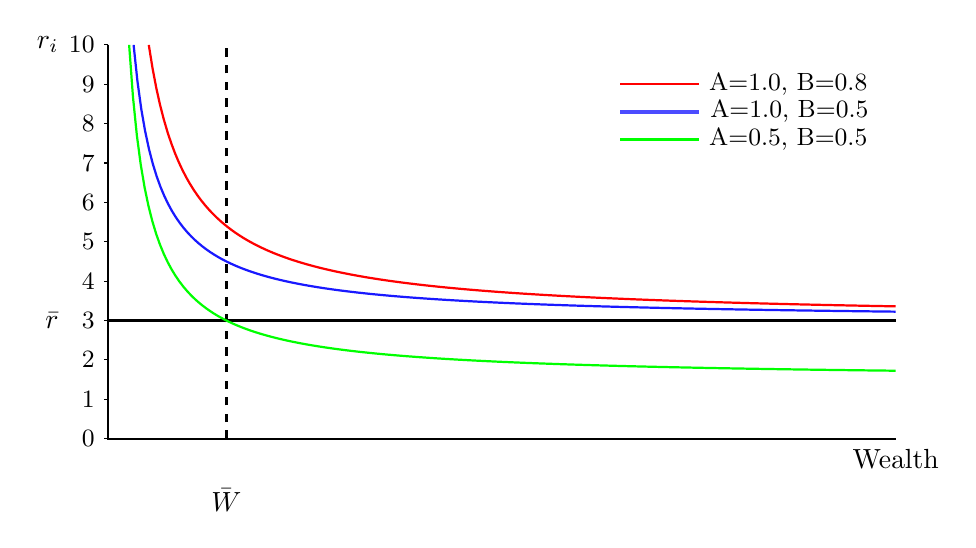
\begin{tikzpicture}[scale=.5]
%\def\bndmax{5} % https://tex.stackexchange.com/questions/68462/filling-a-complex-region-with-tikz
%\def\bndmin{0.2}
\def \Y {10}    % height of y axis as a pecent
\def \W {20}    % length  of x axis
\def \Wbar {3}  % mean wealth
\def \rbar {3}  % the prime rate 

% Equation   \[ r_i = (A + .5 \frac{\bar{W}}{W_i})\omega\]
\def \Wmin{.63}  %This sets the lower limit fo the 
\def \Wmin{(\B*\Wbar)/(\Y/\rbar-\A)} %function to keep in in bounds
\tikzset{func/.style={thick}}	

% Axes
\draw [thick] (0,\Y)node[left=.5cm]{$r_i$} -- (0,0)--(\W,0)node[below]{Wealth};  
\foreach \yi in {0,...,\Y} \draw (0,\yi)--(-.1,\yi)node[left]{\small$\yi$};
\draw [thick] (0,\rbar)node[left=.5cm]{$\bar r$} -- (\W,\rbar);  	% Axes
\draw [thick,dashed] ( \Wbar,0)node[below=.5cm]{$\bar{W}$} -- (\Wbar,\Y);  	% 

\def \A {1.0}  \def \B {0.5} %BLUE
\draw[func,domain=\Wmin:\W, color=blue!90] plot [samples=200] (\x,{(\A+\B*\Wbar/\x)*\rbar});
\draw [ultra thick, color=blue!70 ](13, 8.3)--(15,8.3)node [right, black] {\small A=\A,\ B=\B};

\def \A {0.5} 
\def \B {0.5} % GREEN
\draw[func,domain=\Wmin:\W, color=green] plot [samples=200] (\x,{(\A+\B*\Wbar/\x)*\rbar});
\draw [thick,  color=green](13, 7.6)--(15,7.6)node [right, black] {\small A=\A, B=\B};

\def \A {1.0}  \def \B {0.8} % RED
\draw[func,domain=\Wmin:\W, red] plot [samples=200] (\x,{(\A+\B*\Wbar/\x)*\rbar});
\draw [thick,  color=red](13, 9)--(15,9)node [right, black] {\small A=\A,\ B=\B};
% KEY
\end{tikzpicture}
\caption{Individual borrowing cost as a function of wealth}
\label{Fig:Borrowingrate1}
\end{figure}


\begin{figure}
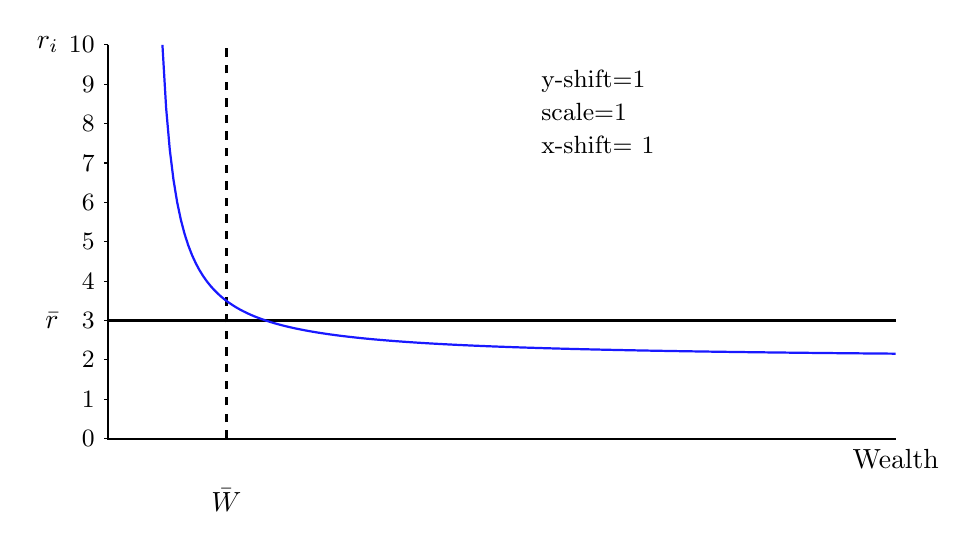
\begin{tikzpicture}[scale=.5]
%\def\bndmax{5}        %https://tex.stackexchange.com/questions/68462/filling-a-complex-region-with-tikz
%\def\bndmin{0.2}
\def \Y {10}  % height of y axis pecent
\def \W {20}  % length  of x axis
\def \Wbar {3} % meam wealth
\def \rbar {3}% this is the prime rate 

%\def \Wmin{(\B*\Wbar)/(\Y/\rbar-\A)} %function to keep in in bounds
\tikzset{func/.style={thick}}	
	% Axes
\draw [thick] (0,\Y)node[left=.5cm]{$r_i$} -- (0,0)--(\W,0)node[below]{Wealth};  
\foreach \yi in {0,...,\Y} \draw (0,\yi)--(-.1,\yi)node[left]{\small$\yi$};
\draw [thick] (0,\rbar)node[left=.5cm]{$\bar r$} -- (\W,\rbar);  	% Axes
\draw [thick,dashed] ( \Wbar,0)node[below=.5cm]{$\bar{W}$} -- (\Wbar,\Y);  	% 

\def \A {1} %vertical shift aroung \rbar, the prime rate
 \def \B {1}  % Scales the exponential curveBLUE
 \def \C {1}  %right shift  
% \def \Wmin {.4+\B}  %This sets the lower limit fo the 
\def \Wmin {(\B*\Wbar)/(\Y-\rbar+\A) +\C} %function to keep in in bounds

\draw[func,domain=\Wmin:\W, color=blue!90] plot [samples=200] (\x,{\rbar-\A+\B*\Wbar/(\x-\C))});
\node  [align=left, text width =2cm ] at (13, 8.3) {\small y-shift=\A \newline scale=\B \newline x-shift= \C};

 \end{tikzpicture}
\caption{Individual borrowing cost as a function of wealth II}
\label{Fig:Borrowingrate2}
\end{figure}

The rates $\delta,\ \sigma,$ and $r$ depend on the period, $T$. 

\section{Incorporating growth and discounting}
%We need a time period T for calculations. For use in any calculation, 

With a price-growth rate of $\dot P$ per year, the growth over $T$ years is $(1+\dot P)^T$, and  %and a 5 year mortgage period, 
the expected price at the end of the period is:

\[P^e_T=P_0(1+\dot P)^T\]

If, for example price growth is 10\%, $\dot P= 0.1$, the {capital gain}, or growth, over a 5-year mortgage term is 0.61051 $\approx$ 60\% of the original price, $P_0$.

If we want the compounded interest rate person $i$ the term T,
\[r_i^T=(1+r_i)^T\]
% This is the value we use in equation~\ref{EqBidPrice}.

If person $i$  discounts at a discount rate $r^\delta$, the present value of a receipt at time $t$ is calculated by using the \textbf{discount factor} $\delta_i^T$.

\[\delta_i^T= \left( \frac{1}{1+r_\delta} \right)^T \]
%\[\delta_i^T= \sum_{\tau=0}^{\tau=T}\left( \frac{1}{1+r_\delta} \right)^\tau \]
 
These can be combined into a function %\delta that  gives a single discounting factor  for a value  like future price that is both growing and being discounted over several (T) periods:
\[ PDV(P^e_T)=P_0\left( \frac{1+\dot P}{1+r_\delta} \right)^T \]
This PDV function specifically combines any expected rent increase, the individual's discount rate and the mortgage term into a single operation.

\subsection{Mortgage availability}
For home loans, many personal finance experts recommend total housing costs account for less than 28\% of your \textbf{gross} household income, This gives us an \textbf{income-based  mortgage maximum} of \[M^{max}_Yi = \frac{0.28*(\omega+w)}{r_i}\] It is the maximum the bank will let you pay.

We assume $r_i$ is based on the individual's assets, on relative wealth. Where is it calculated for the householder or the bank?

We get a \textbf{price-based mortgage maximum} \[M^{max}_P = 0.8P_0\] where $P_0$ is the actual sale price. This is based on the maximum amount of risk that the bank is willing to take on. ($P_0$  will not always be the same as the asking price or the warranted price.)



\section{WHERE DOES THIS GO? Calculate rate of return for an investor}

 The warranted price of the property is the present value of the \gls{warranted rents}% *** Note the warranted price may be rising. This is a problem for  us. WHY?
% NOTE Some of the taxes and most of the repairs/maintenance costs are for the building and not the for the locational value of the land. These two have correlated values. (we can't separate the amount of house and quality form our locational decision ) 

%**** We would like to  somehow ignore the building and push it into the subsistence wage. Can we do this? EXPLAIN
% How do we ignoor buildings - when we talk about the land rents, we're calculating on the basis of the warranted rent wage premium- put people are paying for buildings.. - assume it comes out of the subistence wage- since this is just a theoretical treatment.-- but if you think about how much capital gain will you get, we'll also get capital gainso on the house piece which is not locational- just gains on that asset they happen to have.. --  looking at things coming from close toe the center ignoring what else. - tied together so market spreads capital gain over both of them, and the tax does the same too-- for locational advantage and services..

% Since the present value of rental income (OR NET RENTAL INCOME?) is the value of the house, i.e.,\\

In principle, the  sale price of a unit of land considered is the present discounted value of the stream of net rents. If $\mathcal{R}_N$ is one period rent, which is conventionally calculated as:
\begin{equation}
  P=\frac{\mathcal{R}_N}{r}  
\label{eq:Capitalization}
\end{equation}

%\[v= \delta(P^T- (1+r)M)    +\phi\mathcal{R}\]

*** CLARIFY WHAT WE GET FROM INCLUDING $\psi$, and define, maybe compare with other shares like $\phi$.

\noindent so we can write 

\begin{align}  
    V & = \delta \left((1+\dot P)  P_0- (1+r)mP_0 \right)  + \psi rP_0  \\
      & =\left( \delta ((1+\dot P)  - (1+r)m)\  + \psi r\right)P_0
\end{align}
%there are potetntilaly two interest ratex hereee - one used for capitaliΩing rents to price, and one  is $r_i$. It may be sensibe to use the same value for both. Person I might be looking at the actual rents and using them to calculate the prtice it should sell for. If there is a real estate agent providing price information the tory may be different. SWe are really using htis for the expected value of the present value of net rent, and 

This can be expressed in terms of the rate of return on the down payment, $V/D$
\begin{align*}  
v & = \frac{V}{D} \\
  & = \left( \delta ((1+\dot P) - (1+r)m)\ + \psi r\right)P_0/D \\
  & = \left( \delta ((1+\dot P) - (1+r)m)\ + \psi r\right) \frac{P_0}{P_0-mP_0} \\
  & = \frac{ \delta \left((1+\dot P) - (1+r)m\right)\ + \psi r}{1-m}
\label{eq:RULE}
\end{align*}
